\documentclass[a4paper]{article}
\usepackage[english]{babel}
\usepackage[utf8]{inputenc}
\usepackage{alltt,amsmath,hyperref,graphicx}
\usepackage[usenames,dvipsnames]{xcolor}

% Link colors
\hypersetup{colorlinks=true,linkcolor=black,urlcolor=blue,citecolor=OliveGreen}

% Set paragraph indentation
\parindent 0pt
\parskip 1.0ex plus 0.5ex minus 0.2ex

\title{Internet Programming - Assignment 1}
\author{Jayke Meijer, 2526284, jmr251, \url{jayke.meijer@gmail.com}}

\begin{document}

\maketitle

\tableofcontents
\pagebreak

\section{Used platform}

All code is tested and executed on a machine running Ubuntu 12.04. The used version of
\emph{gcc} is 4.6.3. The JDK used is OpenJDK IcedTea6 1.11.4. The Java version is
1.6.0\_24.

\section{Writing a Micro-Shell}

The first exercise of assignment 1 is to write a number of shell programs and to answer
some questions about them.

\subsection{mysh1}

The first shell reads a command and executes it. The command does not yet have arguments.
To be able to do this, once the command is read and verified, the process forks. The child
process than proceeds to execute the command using \texttt{execlp()}. The parent waits for
the child to complete, than asks for a new command.

\subsection{mysh2}

Mysh2 is an extension of the first shell. It is capable of handling execution of programs
with arguments. The command string is split on spaces. Each of the arguments is put in an
array, and the execution is started using \texttt{execvp()}, which has the ability to pass
a NULL-terminated array to the executed program as ``commandline''-arguments.

\subsection{mysh3}

The third shell supports a piped operation. Two processes are started, and the output of
the first is the input of the second. For example, the command \texttt{ls /tmp | wc -l} 
has to be possible.

This means the command has to be split first. If no pipe is required, execution is like in
mysh2. Otherwise, there are two design possibilities. The parent has to fork a child that 
will start the first process. That child can than fork the second child process, that
will execute the second program. The other option is that the second child is spawned by
the initial parent process. See also figure \ref{tree}.

\begin{figure}
    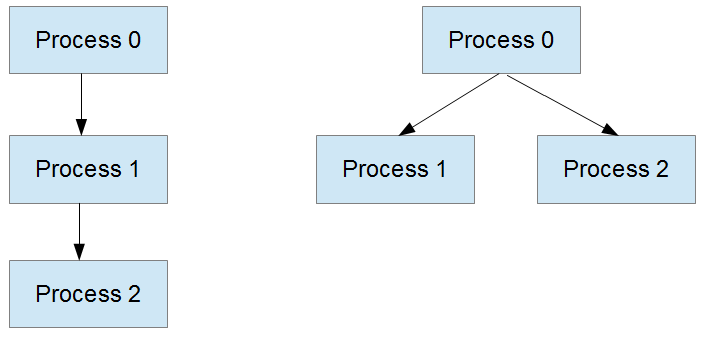
\includegraphics[scale=.5]{img/tree.png}
    \caption{The two design options. Process 0 can spawn just process 1, which in turn 
        spawns process 2, or process 0 can spawn both child processes.}
    \label{tree}
\end{figure}

The second option is used in this program. This allows the parent to create the second
process while the first is initializing itself. It also is more true to what seems to 
happen, the parent `owns' both programs, the first child does not own the second. The 
third advantage is that the parent now knows the process id of both children, allowing it
to wait until both children are finished.

\subsection{Answers to the questions}

\begin{itemize}
    \item \textbf{Question A} The process must create three processes: The parent, the 
            first child program and the second child program. One pipe has to be created,
            because there only has to be one-directional communication: the output of the
            first process to the input of the second. The shell has to wait until both
            child processes are finished before being able to accept another command.
    \item \textbf{Question B} You can not implement a shell program that uses threads
            instead of processes. To be able to execute a new process, the \texttt{exec()}
            call has to be used. This call takes over the entire process. Since threads
            are all part of the same process, this will end all threads of the shell 
            program, effectively killing the shell.
    \item \textbf{Question C} No, this is not possible. \texttt{cd} is part of the 
            original shell and changes value there. Since a child cannot alter the state
            of its parent, \texttt{cd} is not possible in the shell that was written for 
            this assignment.
\end{itemize}

\subsection{Optional}

The command \texttt{cd} is added to \texttt{mysh3}. It uses \texttt{chdir} to change the
current working directory.

\section{Synchronization}

\subsection{Part a}

The program simultaneously writes the sentences "Hello world" and "Bonjour monde", one
character at a time. It does this by forking. The child created by this fork prints the
first sentence, the parent the second.

There is no synchronization, so both messages will be printed at the same time, which
means the messages will be mixed up.

\textbf{Question D} Mutual exclusion is needed. Only one of the process can access the
\texttt{display} function at a time. This will ensure that the message of one of processes
is printed before the other can start printing. The primitive needed for this to work is a
lock. A lock will ensure that once a process has entered a certain part of code (the
\emph{critical section}). If another process tries to enter that piece of code, it is 
forced to wait until the first process is done.

A lock has two functions, \texttt{lock()} and \texttt{unlock()}. When you want to enter 
the critical section you call the \texttt{lock()} function. This will either allow you to
enter or block until you are allowed to enter. Once you are done you call
\texttt{unlock()} and the lock is released. Other processes are now allowed to enter (one
at a time of course).

The program \texttt{syn1} does this. As a lock, a semaphore is used. By decreasing the 
value of the semaphore to zero the display function is locked. Another process trying to
decrease the value of the semaphore sees that it is already zero and it will wait until 
the first process increases the semaphore again, so the second thread is now allowed to
lower it and enter the critical section.

\subsection{Part b}
\textbf{Question E} In this exercise both processes have to ``cooperate'' to print the
proper message. This means that the lock mechanism used in the previous exercise is not
applicable here. The lock only ensures that the processes do not print simultaneously, but
does not guarantee an order in which this happens.

The proper synchronization variable to use is a flag, or more specifically two. These 
flags allow synchronization between the processes, not just mutual exclusion.

When the first process has printed \texttt{``ab''}, it raises flag 1 to signal to process
two that it should now print \texttt{``cd\textbackslash n''}. It then waits for flag 2 to
be raised.

Process two waits for the flag of process one to be raised. When it is raised, it prints
the string, lowers flag 1 and raises flag 2. Then it waits for flag 1 to be raised again.

This way, the processes take turns printing, ensuring that the order in which they print
is as required.

This is done in the program \texttt{syn2}. As flags, two semaphores are used. When the 
semaphore is zero the flag is down and a process can ``raise'' it by increasing it to one. 
The other process can wait while the flag is down and only proceed when it is raised, ie 
the semaphore is increased to one.

\subsection{Part c}

The first program written is \texttt{synthread1}. This is a C program that implements the
correct version of \texttt{syn1}, using pthreads.

For this program the synchronization is provided by a \texttt{pthread\_mutex}. This is a 
lock mechanism, that can be locked with the functions \texttt{pthread\_mutex\_lock()} and
unlocked by \texttt{pthread\_mutex\_unlock()}. The mutex is a global variable to ensure it 
is available in both threads. The threads call the lock method right before calling the
display function and the unlock after display has returned. This ensures only one of the
threads enters the display function at a time.

The second program is \texttt{synthread2}. This C program is the correct implementation of
\texttt{syn2}.

In the answer to question E it was said two flags are needed. The actual implementation is
slightly different, but the principle remains. As ``flags'' two semaphores are used. These
semaphores do not have a lower and raise like a flag, but only have a \texttt{sem\_post()}
function. This function increases the value of the semaphore by one. A thread that has to
wait until ``the flag is raised'', will wait until the value of the semaphore is 
increased. The idea of raising the flag (increasing the semaphore) remains, but lowering 
the flag is no longer required.

\textbf{NOTE:} The assignment said no changes to the function display are allowed. 
However, I have made one change, which is to check the return value of the write function.
This to make sure the compiler does not generate any warnings. This has no affect on the
actual functioning of this function or the output that is generated by this function.

\subsection{Part d}

For this part of the assignment, the programs as shown in part c have to be rewritten in
Java, using Java threads.

The first program is \texttt{syn1.java}. This works like \texttt{synthread1}. As mutual
exclusion mechanism the monitor of a variable is used. This variable is called 
\texttt{lock} in the code. The execution of the critical section (the function display)
is now placed within a synchronized block, ie: \\\texttt{synchronized (lock) \{ 
display(...); \} }\\
This provides mutual exclusion, as long as each call to display is contained by a 
synchronised block using the same variable.

Note that making the function display itself synchronized, ie \texttt{synchronized 
static public void display()} would also work. However, the assignment stated that display
should not be changed.

The second program is the Java version of \texttt{synthread2}. As semaphore once again the
monitor functionality of a variable is used. There are two variables, \texttt{sem1} and
\texttt{sem2}. These are not really semaphores, but are called sem to show the parallels 
with the C program. Instead of waiting until the value of the semaphore is raised, we now
wait until a notification on the object is given. This can be done by calling 
\texttt{sem1.wait()}. This notification is given by \texttt{sem1.notify()}. Since there is
only one other thread, \texttt{notifyAll()} is not required (but would not be wrong).

To run the Java programs, the scripts ``run\_syn1'' and ``run\_syn2'' are available.

\end{document}